%\begin{figure}[h]
%    \centering
%	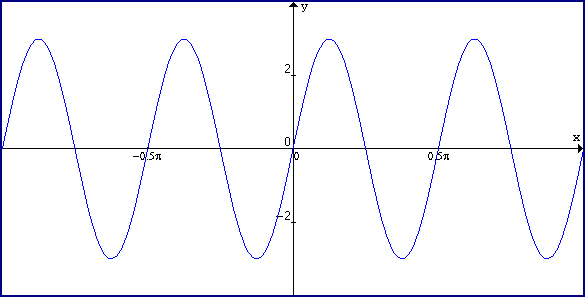
\includegraphics[scale=0.5]{graph}
%	\caption{An example graph}
%	\label{fig:x sine graph}
%\end{figure}

To perform the actual event detection, we propose two algorithms. The first one is a modification of the greedy approach introduced by \cite{event-detection}, which forms events by greedily minimizing temporal and semantical distance of words. We build on top of this algorithm to incorporate the word embeddings as well as alter the temporal distance measure.

The second approach interprets events as literal clusters of words and uses a clustering algorithm to obtain them, rather than explicit cost minimization.

In this section, we describe both algorithms, which we will later compare.


\section{Greedy approach}
This algorithm works by grouping word features together by greedily minimizing a cost function representing their temporal and semantic distance. We will first define a distance measure in each of these domains, combine them into the cost function and then describe the algorithm itself.

An event will be represented by a set of keywords. In each iteration, the keyword closest to the event built so far will be added to that event. We will therefore need to measure the distance between a word feature and a whole set of features.

\subsection{Measuring trajectory distance}
After normalization to sum up to 1, the trajectory $\vect{\traj}_{f}$ of a word feature $f$ can be interpreted as a probability distribution over days, with $\traj_{f}(i)$ denoting the probability that a random document published on day $i$ will contain the word feature $f$. This interpretation allows us to compare the trajectories using information-theoretic techniques, notably the information divergence.

Given a set of word features $\featset$ and another feature $f$ with all trajectories normalized to probabilities, the temporal distance of $f$ to $\featset$ is

\begin{equation}
	\trajdist( \featset, f ) \coloneqq \kl{\vect{\bar{\traj}}_{\featset}}{\vect{\traj}_{f}},
\end{equation}

where $\vect{\bar{\traj}}_{\featset}$ is the mean of all trajectories of features in $\featset$, $\vect{\traj}_{f}$ is the trajectory of feature f and $\kl{\cdot}{\cdot}$ denotes the Kullback-Leibler divergence.


\subsection{Measuring semantic similarity}
Most of the astounding results of the word2vec model come from semantic relations between words being preserved under vector arithmetic, with words concerning the same topic forming clusters. However, as the topic space is high-dimensional, traditional Euclidean distance would vary greatly between different words. Therefore, we use cosine similarity instead, which is bounded in $[-1, 1]$ and independent on the vector lengths. The cosine similarity is a measure often used in information retrieval: \cite{cosine-similarity-i, cosine-similarity-ii}.

Note that we use cosine \textit{similarity} rather than \textit{distance}, which is simply a mean to respect the structure proposed by \cite{event-detection}, who used a simpler measure of document overlap, and the cost function will be constructed accordingly.

Given a set of word features $\featset$ and another feature $f$, the semantic similarity of $f$ and $\featset$ is

\begin{equation}
	\semsim( \featset, f ) \coloneqq \frac{\inp[\big]{\bar{\embed}_{\featset}}{\embed_{j}}}{\| \bar{\embed}_{\featset} \| \cdot \| \embed_{j} \|},
\end{equation}

where $\bar{\embed}_{\featset}$ is the mean of all vector embeddings of features in $\featset$ and $\embed_{f}$ is the vector embedding of the feature $f$. Here, the mean vector is supposed to represent a shared topic among words from $\featset$.


\subsection{Cost function}
Intuitively, an event should be represented by keywords highly correlated in the time domain, concerning the same topic, and with high enough power to be considered representative.

A cost function incorporating all these requirements is therefore defined as

\begin{equation} \label{eq:cost-function}
	\cost( \featset, f ) \coloneqq \frac{\trajdist( \featset, f )}{\exp(\semsim( \featset, f )) \cdot \sum_{g \in \featset \cup f}{\text{DPS}_{g}}},
\end{equation}

where we exponentiate the cosine similarity so that the resulting value is always positive. As the algorithm will minimize this function, the resulting events will have low trajectory divergence, high semantic similarity will consist of important keywords.


\subsection{Event detection}
To perform the event detection itself, we mostly adapt the \textit{Unsupervised greedy event detection} algorithm from \cite{event-detection}. We do make a change in the initial sorting and sort the word features in \textit{ascending} rather than descending order. This ensures that words with lower DPS value will get selected first and that the cost function will not be minimized as quickly. As a result, the events will contain more representative keywords. This effectively relaxes the DPS part of the cost function while keeping emphasis on the trajectory distance and semantic similarity.

\begin{algorithm}[H]
\begin{algorithmic}[1]
\caption{Unsupervised greedy event detection}
\Input $\text{Feature set} ~ F = \text{HH or HL}$

\State $\text{Sort the features in ascending DPS order: } DPS_{f_{1}} \leq \dots \leq DPS_{f_{\left\vert F \right\vert}}$

\State $k = 0$

\ForEach{$f \in F$}
	\State $k = k + 1$	
	\State $e_{k} = \{ f \}$
	\State $cost_{e_{k}} = \frac{1}{DPS_{f}}$
	\State $F = F \setminus f$
	
	\While{$F \neq \emptyset$}
		\State $m = \argmin\limits_{m}{\cost( e_{k}, f_{m} )}$

		\If{$\cost( e_{k}, f_{m} ) < cost_{e_{k}}$}
			\State $cost_{e_{k}} = \cost( e_{k}, f_{m} )$
			\State $e_{k} = e_{k} \cup f_{m}$
			\State $F = F \setminus f_{m}$
		\Else
			\Break
		\EndIf
	\EndWhile
\EndFor

\Output $\text{Events} ~ \{ e_{1}, e_{2}, \dots, e_{k} \}$
\end{algorithmic}
\end{algorithm}


\section{Cluster-based approach}


\section{Event detection}
To cluster the word features in both time and semantic domains, we will need to measure their distance. We first define a pairwise distance measure in each domain. These measures are then generalized to measure the distance of a feature from a whole set of features, so we can assign the closest feature to a partially constructed event. In the last step, these distances are combined into a single cost function which we aim to minimize.


\subsection{Measuring trajectory distance}

Distance between two feature trajectories is defined in terms of their information divergence. Unlike \cite{event-detection}, we use the \textit{Jensen-Shannon} divergence:

\begin{equation*}
	\featsim( \vect{p} \| \vect{q} ) = \frac{1}{2} \text{D}( \vect{p} \| \vect{m} ) + \frac{1}{2} \text{D}( \vect{q} \| \vect{m} ),
\end{equation*}

where $\vect{m} = \frac{1}{2} \left( \vect{p} + \vect{q} \right)$ and $\text{D}( \cdot \| \cdot )$ denotes the \textit{Kullback-Leibler} divergence.



{\color{red} TODO: Move the pairwise similarities to the cluster-based algorithm, keep only the set-feature ones here.}

{\color{blue} TODO: Try KL(mean(M),f) instead of JSD(mean(M),f)? Like M is the true distribution and f assumed. Keep JSD in pairwise similarity though, clustering likes symmetry.}


\subsection{Measuring semantic similarity}

The semantic similarity is again first defined for two features, and then generalized to a similarity between a feature set and another feature. Here, we utilize the word embeddings computed in \ref{word-embeddings}.

Most of the astounding results of the word2vec model come from semantic relations between words being preserved under vector arithmetic, with words concerning the same topic having roughly the same angle. Thus, we use the cosine similarity between embeddings $\embed_{i}$ and $\embed_{j}$ of word features $i$ and $j$:

\begin{equation}
	\semsim( f_{i}, f_{j} ) \coloneqq \frac{\inp[\big]{\embed_{i}}{\embed_{j}}}{\| \embed_{i} \| \cdot \| \embed_{j} \|}
\end{equation}

Next, we generalize the similarity for a feature set $\featset$ and another feature $f$ as

\begin{equation}
	\semsim( \featset, f ) \coloneqq \frac{\inp[\big]{\bar{\embed}_{\featset}}{\embed_{j}}}{\| \bar{\embed}_{\featset} \| \cdot \| \embed_{j} \|},
\end{equation}

where $\bar{\embed}_{\featset}$ is the mean of all vector embeddings of features in $\featset$ and $\embed_{f}$ is the vector embedding of the feature $f$. Here, the mean vector is supposed to represent a shared topic among words from $\featset$.